\chapter{Performance Simulation Environment}
\label{chapter:performance-simulation-environment}

This chapter describes Performance Simulation Environment (PSE) and its usage for performance analysis of a stream computing system. We begin with an overview of PSE tools and concepts, and continue by describing the three components that describe a PSE model. After that, we go through the simulation and monitoring of PSE applications. Finally, we address the problems and deficiencies, namely the lack of global queue scheduling, that needed to be resolved before PSE could be used for performance analysis of a stream computing system.

\section{PSE Overview}
\label{sec:pse-overview}

PSE is a toolset and simulation environment for dynamic performance analysis of, initially designed but not limited to, parallel computing systems. The tools consist of graphical model editors, compiler tools, and discrete event simulator runtime.

\begin{figure}[ht]
  \begin{center}
    %% \input{images/pse-toolset.tex}
    \missingfigure{\Huge pse toolset overview}
    \caption{PSE toolset includes the model editors, compiler tools and the simulator runtime libraries.}
    \label{fig:pse-toolset}
  \end{center}
\end{figure}

The graphical model editors -- workload editor, wle; task graph editor, tge; sequence chart editor, sce; and resource network editor, rne -- are used to build and edit the PSE model representation of a system. Each model editor has a corresponding compiler (wlc, tgc, scc, and rnc), that is used to compile the textual model representations into C-code.

The generated model code and the built-in simulator runtime libraries are compiled into an executable simulator program, using generic C compiler such as GCC \cite{stallman:2009:gcc}. The resulting program can be run on top of Linux operating system on commodity hardware.

\todo[inline]{yadayada}
\todo[inline]{What can be modeled?? What can't be?}
\todo[inline]{Reusability}
\todo[inline]{Model represents a system.}
\todo[inline]{In PSE, the simulation model is created by graphical user interfaces. Internally the model is presented as a simple text format that is then parsed by tgc.}

\section{PSE Model}

In PSE, the system under study is modeled as a resource network \cite{Menasce:1994:CPP:174466}. The complete model consists of three main components: resource provision model, resource usage model and workload model. Each of the components are presented as directed graphs, where the nodes represent model entities and the arcs represent the possible flow directions of the tasks.

The resource provision model represents the available system resources, for example a computer hardware. The graph nodes represent resource entities, and arcs represent the possible usage order of the resources. The resources are consumed by the tasks generated by the workload model.

A resource can be either active or passive. Active resources provide service and introduce service delay to the tasks using them. An example of active resource could be a processor core, which can serve certain amount of processing cycles per unit time. Passive resources do not induce direct delay to the jobs, but their possession is required to access certain other resources. Locks \todo{cite something} could be an example of passive resource.

\begin{figure}[h!]
  \begin{center}
    \missingfigure{\Huge resource provision model?}
    % \includegraphics[width=\textwidth]{images/.pdf}
    \caption{An example of resource provision model.}
    \label{fig:resource-provision-model}
  \end{center}

\end{figure}

Figure \ref{fig:resource-provision-model} presents an example of a resource provision model ...
\todo[inline]{Explain the figure}

The resource usage models can represented as message sequence charts or tasks graphs. We omit the discussion of the sequence chart in this thesis. A task graph is a representation of the resource usage of the tasks arriving to the system. The nodes in the task graph can be divided into three categories: execution nodes describe the resource usage events and activities, branching nodes conditionally guide the tasks through the graph, and fork/join nodes represent task subdivision. The arcs represent the flow of control in the system.

\begin{figure}[h!]
  \begin{center}
    \missingfigure{\Huge resource usage model?}
    % \includegraphics[width=\textwidth]{images/.pdf}
    \caption{An example of resource usage model.}
    \label{fig:resource-usage-model}
  \end{center}
\end{figure}

Figure \ref{fig:resource-usage-model} presents an example of a resource usage model ...
\todo[inline]{Explain the figure}

The workload model generates tasks, which traverse through the system according to the rules defined in the resource usage model, consuming the resources defined in the resource provision model. The nodes in the workload graph describe the task generating processes, and the arcs define the relationships between them. The graph representing the workload model must be acyclic.

The event spawn rate can be constant or random (specified for example with probability distribution).

When an event is spawned, it progresses through the resource provision model triggering the resource usages. -> gets delayed.

\section{PSE Tools}

\todo[inline]{Should the tools be described in more detail, or should this section be omitted?}

\begin{figure}[h]
  \begin{center}
    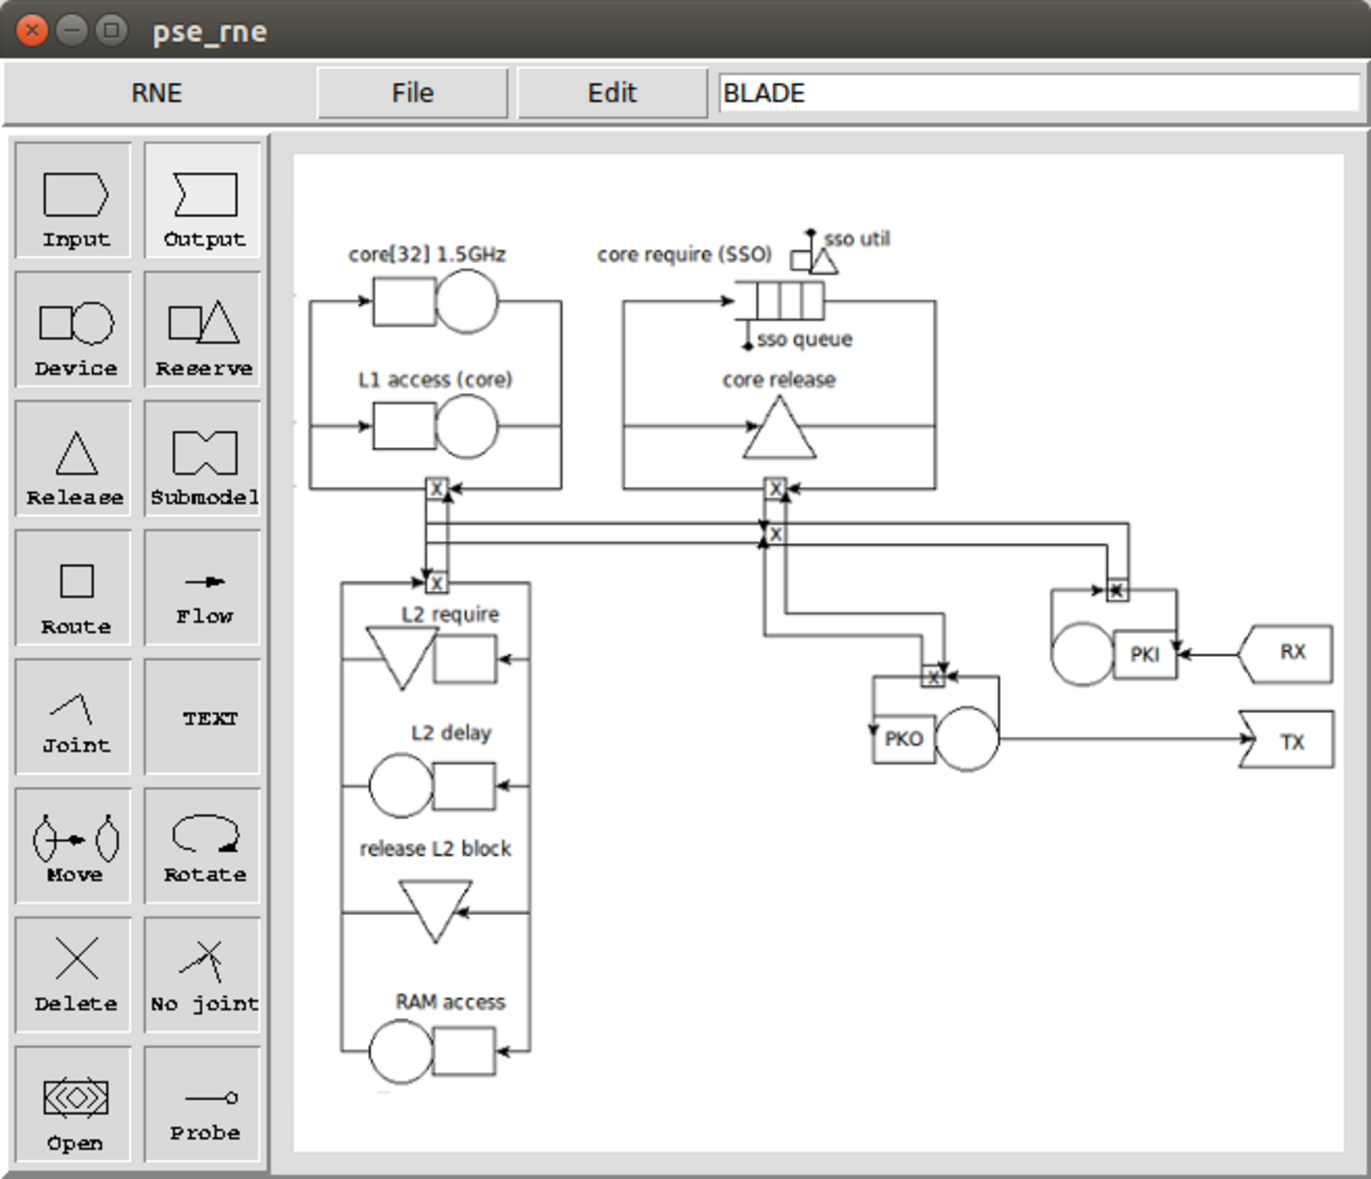
\includegraphics[width=\textwidth]{images/rne-example.pdf}
    \caption{The graphical user interface of the resource network editor. The actual resource network model is presented in the middle, and the toolbar on the left.}
    \label{fig:rne-example}
  \end{center}
\end{figure}

\section{Monitoring}

\todo[inline]{Correct place for this?}
The probes can be used to capture every state change of the system.

% - Events from workload model
%   - Workload model creates new events with the event spawn rate described by the user

% - Each event starts by ``entering'' the resource usage model
%   - e.g. calls the function bound to the resource usage model that the user has provided as the JOB-parameter.

% - resource usage model is a set of functions generated by the tgc-compiler from the user created task graph file.
% - resource usage model calls the functions provided by the RNS api -> service delays

% - Active resources call RNS_demand_device or RNS_use_device, which induces a delay
%   - The resource reserved for the time the process is delayed

% - Passive resources reserve the resources using RNS_reserve_resource function
%   - Release happens when the event arrives at the function corresponding the release node specified in the resource usage network
%   - Unlike in the active resource usage, the resource is held by the event for a time unknown at the reserve time

\section{Resource Network Simulator}
\label{sec:resource-network-simulator}

Performance Simulation Environment provides a discrete event simulator engine, named resource network simulator (RNS). The final simulator program is created by compiling the RNS runtime libraries together with the generated simulation model code. The simulator engine manages the simulation execution, i.e. it tracks the global simulation time, schedules tasks and manages the system monitoring.



The simulator inputs are generated by the workload model, which spawns a new system thread for each generated input. The input can be either control input or the actual workload tasks. The former of these are used for the simulation control, for example changing or resetting the simulation time or monitoring metrics. The latter are the actual task entities presented in section


\subsection{RNS Service Routines}
\label{sec:rns-service-routines}

\lstinputlisting[caption=RNS\_use\_device,
                 label=lst:RNS-use-device]{listings/RNS_use_device.c}

RNS\_use\_device in~\ref{lst:RNS-use-device} reserves the resource, delays the process (i.e. the task) and releases the resource for other processes.

\lstinputlisting[caption=RNS\_demand\_device,
                 label=lst:RNS-demand-device]{listings/RNS_demand_device.c}

RNS\_demand\_device routine in~\ref{lst:RNS-demand-device} is a simple wrapper routine, that converts the demanded service amount (service\_amount) into corresponding service time, based on the device entity speed (d-$\textgreater$speed). It then calls the RNS\_use\_device routine with the resulting service time.

\lstinputlisting[caption=RNS\_reserve\_resource,
                 label=lst:RNS-reserve-resource]{listings/RNS_reserve_resource.c}

\ref{lst:RNS-reserve-resource} summarizes the RNS\_reserve\_resource routine. RNS\_reserve\_resource calls the reserve function bound to the resource entity as explained in section \ref{TODO}. The reserve function assigns the task either in the resource's processing queue or waiting queue. If

If the reserve function assigns the task to the waiting queue, the thread yields the execution to the scheduler.

\lstinputlisting[caption=RNS\_delay\_process,
                 label=lst:RNS-delay-process]{listings/RNS_delay_process.c}
\lstinputlisting[caption=RNS\_release\_resource,
                 label=lst:RNS-release-resource]{listings/RNS_release_resource.c}

\subsection{Simulator Engine}
\label{sec:simulator-engine}




\begin{figure}[ht]
  \begin{center}
    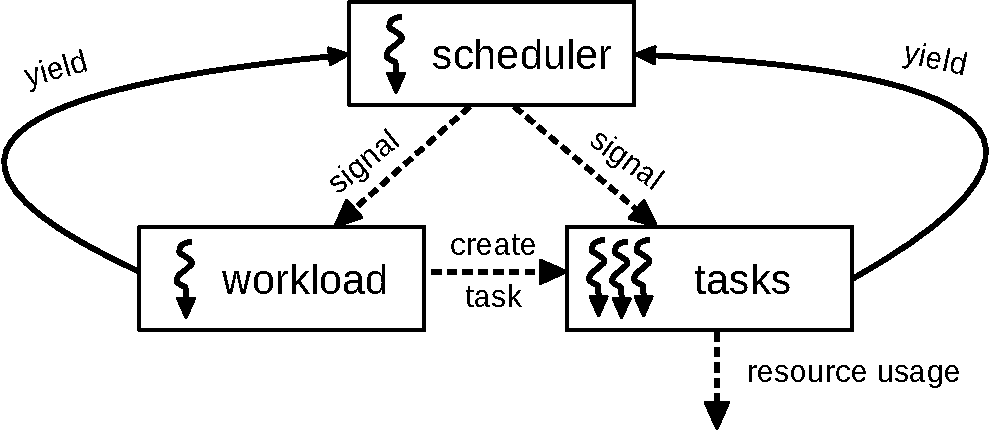
\includegraphics[width=\textwidth]{images/rns-threads.pdf}
    \caption{PSE thread usage}
    \label{fig:rns-threads}
  \end{center}
\end{figure}

RNS advances in the event-advance manner. Each time a thread's task encounters an event that is dependent on the other threads' execution, it yields the execution to the scheduler thread, which then signals the thread with the smallest trigger time.


The thread (task) with the smallest trigger time gets run when the previous running thread has yielded execution.



%%% Local Variables:
%%% mode: latex
%%% TeX-master: "thesis-hartikainen"
%%% End:
